% Originally: content/week-08.tex, \section{Multivariate integration} (Corsin Week 8)

% Source: Corsin Nick/Class Notes/Week 8.pdf, p. 7
\section{Multivariate integration}
\label{sec:multivariate_integration}

% Supplement: Sascha Brack/Class Notes/Week_08_Notes_Monday.pdf, pp. 5--7
\subsection{Jordan measure and the Riemann integral}
The rigorous definition of the multidimensional integral relies on the \newterm{Jordan measure} (\germanterm{Jordan-Maß}). The intuition, as presented in Sascha Brack's notes, involves \qt{dyadic cubes} (pixels) that approximate a region from the inside and outside.

\begin{center}
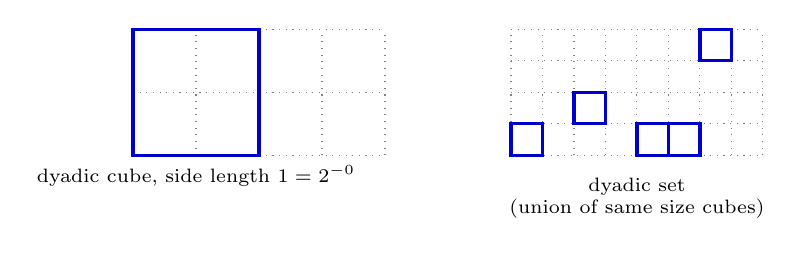
\begin{tikzpicture}[scale=0.8]
  % first grid
  \draw[gray, dotted] (0,0) grid (4,2);
  \draw[very thick, blue!80!black] (0,0) rectangle (2,2);
  \node[below, font=\scriptsize] at (1,0) {dyadic cube, side length $1=2^{-0}$};
  
  \begin{scope}[shift={(6,0)}]
    \draw[gray, dotted, step=0.5] (0,0) grid (4,2);
    \draw[very thick, blue!80!black] (0,0) rectangle (0.5,0.5);
    \draw[very thick, blue!80!black] (1,0.5) rectangle (1.5,1.0);
    \draw[very thick, blue!80!black] (2,0) rectangle (2.5,0.5);
    \draw[very thick, blue!80!black] (2.5,0) rectangle (3.0,0.5);
    \draw[very thick, blue!80!black] (3,1.5) rectangle (3.5,2.0);
    \node[below, font=\scriptsize, align=center] at (2,-0.2) {dyadic set\\(union of same size cubes)};
  \end{scope}
\end{tikzpicture}
\end{center}

% Generator: Claude Opus 5 (High) --- the notion was used throughout this chapter and in
% \cref{ch:change_of_variables} but had no numbered definition to point at.
\begin{definition}[Dyadic cube and dyadic set]
\label{def:dyadic_set}
For $p \in \mathbb{N}$ and $a \in \mathbb{Z}^n$, the \newterm{dyadic cube}
(\germanterm{dyadischer Würfel}) of generation $p$ at $a$ is
\[Q_p(a) := 2^{-p}\big(a + [0,1)^n\big),\]
a half-open cube of side length $2^{-p}$. A \newterm{dyadic set} (\germanterm{dyadische Menge})
is a finite union $E = \bigcup_{\ell=1}^N Q_p(a(\ell))$ of distinct dyadic cubes \emph{of one
common generation} $p$, and its volume is
\[\mu(E) := 2^{-pn}N.\]
\end{definition}

The requirement that all cubes share a generation is not cosmetic: it is what separates the
Jordan theory from the Lebesgue theory, as \cref{rem:jordan_vs_lebesgue_sizes} makes precise.

% Supplement: Sascha Brack/Class Notes/Week_08_Notes_Monday.pdf, pp. 5--7
Similar to the 1D Riemann integral, we approximate the volume of a set $E \subseteq \mathbb{R}^n$ using an outer sequence of dyadic sets $G_i \supseteq E$ and an inner sequence $F_i \subseteq E$. If the limits of their volumes coincide as the pixel size $2^{-p} \to 0$, $E$ is \newterm{Jordan measurable}.

Furthermore, the multidimensional integral of a non-negative function $f : A \to \mathbb{R}$ is exactly the $(n+1)$-dimensional Jordan measure (volume) of its hypograph $\Gamma_A(f)$:

\begin{center}
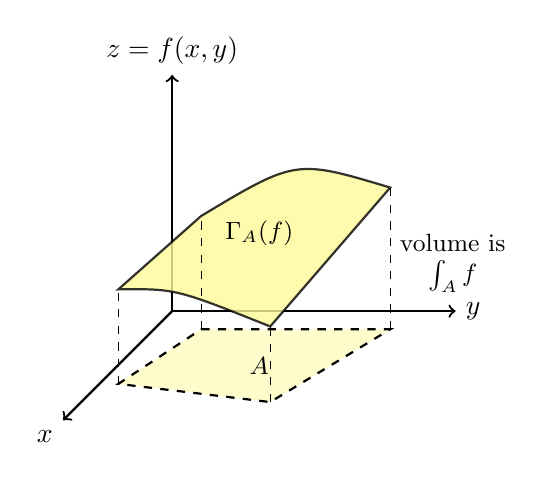
\begin{tikzpicture}[scale=1.2]
  % axes
  \draw[->, thick] (0,0,0) -- (3,0,0) node[right] {$y$};
  \draw[->, thick] (0,0,0) -- (0,2.5,0) node[above] {$z = f(x,y)$};
  \draw[->, thick] (0,0,0) -- (0,0,3) node[below left] {$x$};
  
  % base domain A
  \draw[thick, dashed, fill=yellow!20] (0.5,0,0.5) -- (2.5,0,0.5) -- (2.0,0,2.5) -- (0.2,0,2.0) -- cycle;
  \node[font=\small] at (1.5, 0, 1.5) {$A$};
  
  % top surface graph(f)
  \draw[thick, fill=yellow!40, opacity=0.8] (0.5,1.2,0.5) .. controls (1.5,1.8,0.5) .. (2.5,1.5,0.5)
    -- (2.0,0.8,2.5) .. controls (1.0,1.2,2.5) .. (0.2,1.0,2.0) -- cycle;
  \node[font=\small] at (1.5, 1.4, 1.5) {$\Gamma_A(f)$};
  
  % vertical lines
  \draw[dashed] (0.5,0,0.5) -- (0.5,1.2,0.5);
  \draw[dashed] (2.5,0,0.5) -- (2.5,1.5,0.5);
  \draw[dashed] (2.0,0,2.5) -- (2.0,0.8,2.5);
  \draw[dashed] (0.2,0,2.0) -- (0.2,1.0,2.0);
  
  \node[right, font=\small, align=center] at (2.5, 0.7, 0.5) {volume is\\$\int_A f$};
\end{tikzpicture}
\end{center}

% Source: Jérôme Paschoud/Notizen/Woche 8.2 Riemann-Integral.pdf, p. 1
% Generator: Gemini 3.1 Pro (High)
\begin{definition}[Riemann integral in $\mathbb{R}^n$]
\label{def:riemann_integral_rn}
Let $A \subseteq \mathbb{R}^n$ and $f: A \to \mathbb{R}$. Analogous to Analysis I, the integral is defined via dyadic step functions (\germanterm{dyadische Treppenfunktionen}). The lower and upper integrals are defined as
\begin{align*}
  \underline{\int}_A f &:= \sup \left\{ \int_A g \;\middle|\; g: \mathbb{R}^n \to \mathbb{R} \text{ dyadic step function with } g \leq f \right\}, \\
  \overline{\int}_A f &:= \inf \left\{ \int_A h \;\middle|\; h: \mathbb{R}^n \to \mathbb{R} \text{ dyadic step function with } h \geq f \right\}.
\end{align*}
The function $f$ is \newterm{Riemann integrable} if $\underline{\int}_A f = \overline{\int}_A f$. In this case, their common value is denoted by $\int_A f$.

\begin{center}
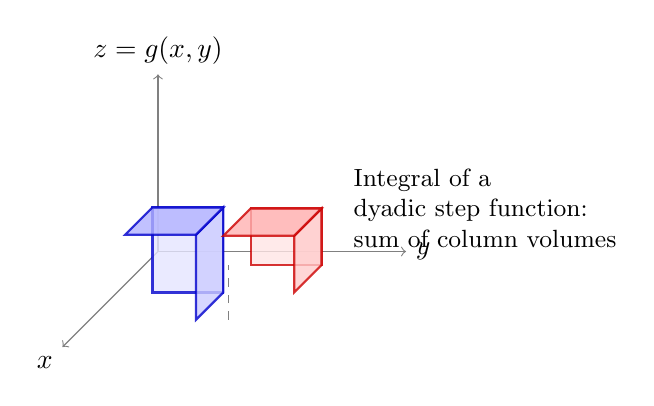
\begin{tikzpicture}[scale=0.9]
  % axes
  \draw[->, gray] (0,0,0) -- (3.5,0,0) node[right, text=black] {$y$};
  \draw[->, gray] (0,0,0) -- (0,2.5,0) node[above, text=black] {$z = g(x,y)$};
  \draw[->, gray] (0,0,0) -- (0,0,3.5) node[below left, text=black] {$x$};
  
  % Base squares
  \draw[gray, dashed] (0.5,0,0.5) grid (2.5,0,2.5);
  
  % Column 1
  \draw[thick, blue!80!black, fill=blue!10, opacity=0.8] (0.5,0,1.5) -- (0.5,1.2,1.5) -- (1.5,1.2,1.5) -- (1.5,0,1.5) -- cycle;
  \draw[thick, blue!80!black, fill=blue!20, opacity=0.8] (1.5,0,1.5) -- (1.5,1.2,1.5) -- (1.5,1.2,2.5) -- (1.5,0,2.5) -- cycle;
  \draw[thick, blue!80!black, fill=blue!30, opacity=0.8] (0.5,1.2,1.5) -- (1.5,1.2,1.5) -- (1.5,1.2,2.5) -- (0.5,1.2,2.5) -- cycle;
  
  % Column 2
  \draw[thick, red!80!black, fill=red!10, opacity=0.8] (1.5,0,0.5) -- (1.5,0.8,0.5) -- (2.5,0.8,0.5) -- (2.5,0,0.5) -- cycle;
  \draw[thick, red!80!black, fill=red!20, opacity=0.8] (2.5,0,0.5) -- (2.5,0.8,0.5) -- (2.5,0.8,1.5) -- (2.5,0,1.5) -- cycle;
  \draw[thick, red!80!black, fill=red!30, opacity=0.8] (1.5,0.8,0.5) -- (2.5,0.8,0.5) -- (2.5,0.8,1.5) -- (1.5,0.8,1.5) -- cycle;

  \node[font=\small, align=left] at (5, 1, 1) {Integral of a\\dyadic step function:\\sum of column volumes};
\end{tikzpicture}
\end{center}

This integral satisfies all the \qt{good} properties from the one-dimensional case, such as linearity. Moreover, if $E \subseteq \mathbb{R}^n$ is Jordan measurable and $f: \overline{E} \to [0, \infty)$ is continuous, then $f$ is Riemann integrable on $E$.
\end{definition}

% Source: Diego Torres Tejeda/Notes - 17.04 - Diego Torres Tejeda.pdf, p. 1
% Generator: Gemini 3.6 Flash (High)
\begin{theorem}[Jordan measurability criterion via boundary]
\label{thm:jordan_measurability_boundary_criterion}
A bounded subset $E \subseteq \mathbb{R}^n$ is Jordan measurable if and only if its boundary $\partial E$ is a Jordan null set, i.e.\ $\mu_{\mathrm{out}}(\partial E) = 0$.
\end{theorem}

\begin{lemma}[Compact sets: Jordan null versus Lebesgue null]
\label{lem:compact_jordan_vs_lebesgue_null}
Let $K \subseteq \mathbb{R}^n$ be compact. Then $K$ is a Jordan null set if and only if $K$ is a Lebesgue null set.
\end{lemma}

\begin{proof}
If $K$ is Jordan null, then for every $\varepsilon > 0$, $K$ is covered by finitely many dyadic cubes $Q_1, \dots, Q_m$ with total volume $\sum_{i=1}^m \mu(Q_i) < \varepsilon$, so $K$ is a Lebesgue null set. Conversely, if $K$ is Lebesgue null, there is a countable cover by dyadic cubes $\{Q_j\}_{j \ge 1}$ with $\sum_{j=1}^\infty \mu(Q_j) < \varepsilon$. Taking the interiors of slightly enlarged cubes yields an open cover of the compact set $K$, which admits a finite subcover of total volume $< 2\varepsilon$, proving $K$ is Jordan null.
\end{proof}

% Source: Diego Torres Tejeda/Notes - 17.04 - Diego Torres Tejeda.pdf, pp. 3--4
% Generator: Gemini 3.6 Flash (High)
\begin{example}[The Cantor set is a Jordan null set]
\label{ex:cantor_set_jordan_null}
Consider the middle-thirds \newterm{Cantor set} $C \subseteq [0,1]$, defined inductively by $C_0 := [0,1]$ and
\[
C_{n+1} := \tfrac{1}{3} C_n \cup \left( \tfrac{2}{3} + \tfrac{1}{3} C_n \right), \qquad C := \bigcap_{n=0}^\infty C_n.
\]
Each $C_n$ consists of $2^n$ closed intervals of length $3^{-n}$, so $\mu(C_n) = (2/3)^n$. Since $C \subseteq C_n$ for all $n$, we have
\[
\mu_{\mathrm{out}}(C) \leq \mu(C_n) = \left(\tfrac{2}{3}\right)^n \xrightarrow{n\to\infty} 0,
\]
proving that the Cantor set $C$ is a Jordan null set.

Moreover, as Diego Torres Tejeda highlights in his notes, $C$ consists precisely of those points $x \in [0,1]$ possessing a ternary (base-3) expansion $x = \sum_{n=1}^\infty \frac{a_n}{3^n}$ composed entirely of digits $a_n \in \{0, 2\}$ without the digit $1$.
\end{example}

% Source: Diego Torres Tejeda/Notes - 17.04 - Diego Torres Tejeda.pdf, p. 5
% Generator: Gemini 3.6 Flash (High)
\begin{example}[An open set that is not Jordan measurable]
\label{ex:non_jordan_measurable_open_set}
Jordan measurability can fail even for open sets. Enumerate the rational numbers in $[0,1]$ as $\mathbb{Q} \cap [0,1] = \{q_1, q_2, \dots\}$, and define the open set
\[
U := \bigcup_{k=1}^\infty B_{2^{-(k+2)}}(q_k) \;\cap\; (0,1).
\]
Since $\mathbb{Q} \cap [0,1]$ is dense in $[0,1]$, the closure of $U$ is $\overline{U} = [0,1]$. If $U$ were Jordan measurable, its measure would satisfy $\mu(U) = \mu(\overline{U}) = 1$. However, any finite union of intervals covering a dyadic inner approximation of $U$ has measure bounded by $\sum_{k=1}^\infty 2 \cdot 2^{-(k+2)} = \frac{1}{2}$. Thus $\mu_{\mathrm{in}}(U) \leq \frac{1}{2} < 1 = \mu_{\mathrm{out}}(U)$, showing that $U$ is \textbf{not} Jordan measurable. Its boundary $\partial U = [0,1] \setminus U$ is a \qt{fat} boundary of positive outer measure.
\end{example}

% Source: Jérôme Paschoud/Notizen/Woche 8.1 Tangentialräume und Jordan Mass.pdf, p. 3
% Generator: Gemini 3.1 Pro (High)
\begin{proposition}[Algebra of Jordan measurable sets]
\label{prop:algebra_jordan_measurable}
If $E, F \subset \mathbb{R}^n$ are Jordan measurable, then their union $E \cup F$, intersection $E \cap F$, and differences $E \setminus F$, $F \setminus E$ are also Jordan measurable.
Furthermore, if $E \cap F = \emptyset$ (or if they only intersect in a Jordan null set), then
\[
\mu(E \cup F) = \mu(E) + \mu(F).
\]
\end{proposition}

% Source: Jérôme Paschoud/Notizen/Woche 8.1 Tangentialräume und Jordan Mass.pdf, p. 4
% Generator: Gemini 3.1 Pro (High)
\begin{remark}[Lebesgue null vs.\ Jordan null]
\label{rem:lebesgue_vs_jordan_null}
A set $E \subset \mathbb{R}^n$ is \newterm{Lebesgue null} if for every $\varepsilon > 0$, there exist \emph{countably} many dyadic cubes $Q_i$ covering $E$ with $\sum \mu(Q_i) < \varepsilon$. For a \newterm{Jordan null} set, the cover must be formed by \emph{finitely} many cubes (which implicitly requires $E$ to be bounded).
Because a countable cover is allowed, the set $\mathbb{Q} \cap [0,1]$ is Lebesgue null. However, it is not Jordan null (in fact, it is not even Jordan measurable, as seen in \cref{ex:non_jordan_measurable_open_set}), since any finite union of intervals covering it must also cover its closure $[0,1]$, thus having measure at least $1$.
\end{remark}

% Quelle: Linus Lüchinger/Slides/Slides-04-16.pdf, slide 6
% Generator: Claude Opus 5 (High)
\begin{remark}[The relaxation is really about \emph{sizes}, not just counts]
\label{rem:jordan_vs_lebesgue_sizes}
Stating the difference as \qt{finitely many} against \qt{countably many} is correct but hides
where the extra power actually comes from. A Jordan cover is a \emph{dyadic set}, and every cube
in a dyadic set of generation $p$ has the same side length $2^{-p}$
(\cref{def:dyadic_set}). So the two conditions really read:
\begin{itemize}
  \item \textbf{Jordan null:} for each $\varepsilon>0$, cover $E$ by cubes that all have
    \emph{one common side length}, of total volume $<\varepsilon$. Finiteness is then automatic:
    only finitely many cubes of a fixed size fit into a bounded region.
  \item \textbf{Lebesgue null:} for each $\varepsilon>0$, cover $E$ by cubes of \emph{whatever
    side lengths you like}, of total volume $<\varepsilon$. Allowing the sizes to vary is exactly
    what lets the cover be infinite while the total volume stays finite.
\end{itemize}
The two relaxations are therefore one relaxation. It is permission to shrink the cubes as you go
that buys the countable cover, and it is the countable cover that makes the notions differ.

$\mathbb{N} \subseteq \mathbb{R}$ shows this in its purest form. Cover the integer $k$ by an
interval of length $\varepsilon\,2^{-k-1}$; the total length is $\varepsilon$, so $\mathbb{N}$ is
Lebesgue null. No Jordan cover can do this: cubes of one fixed length $2^{-p}$ need at least one
cube per integer, infinitely many of them, of infinite total length. (Indeed $\mathbb{N}$ is
unbounded, so it is not Jordan measurable at all.) The point is that the geometric series is
available only when the sizes may vary.
\end{remark}

% Source: Jérôme Paschoud/Notizen/Woche 8.1 Tangentialräume und Jordan Mass.pdf, p. 4
% Generator: Gemini 3.1 Pro (High)
\begin{theorem}[Linear transformations of Jordan measurable sets]
\label{thm:jordan_measure_linear_transformation}
Let $L: \mathbb{R}^n \to \mathbb{R}^n$ be a linear, invertible map. If $E \subset \mathbb{R}^n$ is Jordan measurable, then the image $L(E)$ is also Jordan measurable, and its measure scales by the absolute value of the determinant of $L$:
\[
\mu(L(E)) = |\det L| \, \mu(E).
\]
\end{theorem}


% --- exercises relocated here from the dissolved sheet 8 ---

% Originally: content/week-08.tex, \exercisesheet{8}, problem 8.2
% Source: exercises/Ex8_Analysis2_eng.pdf

% Source: exercises/Ex8_Analysis2_eng.pdf, p. 1
\begin{exercise}[8.2 --- True or False \textnormal{(important)}]
\label{ex:8.2}
\begin{enumerate}[label=\textbf{\arabic*.}]
  \item A bounded countable set is always Jordan-null.
  \item A countable set is always Lebesgue-null.
  \item Let $D \subset [0,1]$ be a dense set (i.e.\ $\overline D = [0,1]$). Then
    $\mu_{out}(D) = 1$. ($\mu_{out}$ was defined in Definition 13.10.)
  \item Let $X, Y \subset [0,1]$ Jordan measurable sets such that $\mu(X) > 1/2$ and
    $\mu(Y) > 1/2$. Then $X \cap Y \neq \emptyset$.
  \item Let $X, Y \subset [0,1]$ such that $\mu_{out}(X) > 1/2$ and $\mu_{out}(Y) > 1/2$. Then
    $X \cap Y \neq \emptyset$.
\end{enumerate}
\textit{Official hint:} \textbf{8.2.5} --- $\mu_{out}$ can be positive and large on very sparse
sets\dots

% Supplement: Sascha Brack/Ex Sheet Hints/Ex8_Analysis2_hints.pdf, p. 1
\textit{Sascha Brack's hints:} a toolkit of sets worth testing every part against ---
$\mathbb{Q}$, the irrationals $\mathbb{R}\setminus\mathbb{Q}$, $\mathbb{Q}\cap[0,1]$, and
$(\mathbb{R}\setminus\mathbb{Q})\cap[0,1]$. For \textbf{8.2.3} specifically: monotonicity already
gives $\mu_{out}(D) \leq \mu_{out}([0,1]) = 1$, so the work is showing
$\mu_{out}(D) \geq 1$ --- essentially, that the \qt{smallest} dyadic set containing $D$ also
contains $[0,1]$.
\end{exercise}

% Originally: content/week-08.tex, \exercisesheet{8}, problem 8.4
% Source: exercises/Ex8_Analysis2_eng.pdf

% Source: exercises/Ex8_Analysis2_eng.pdf, p. 1
\begin{exercise}[8.4 --- Multiple Choice \textnormal{(important)}]
\label{ex:8.4}
Let $U \subset \mathbb{R}^n$ be a nonempty, open subset, $f : U \to \mathbb{R}^m$ a function,
and $N \subset U$ a Jordan null set. In which of the following cases is the image
$f(N) \subset \mathbb{R}^m$ necessarily a null set? \textit{Attention: Only one answer is
correct!}
\begin{enumerate}[label=\textbf{\arabic*.}]
  \item If $f$ is uniformly continuous.
  \item If $f$ is uniformly continuous and $m \geq n$.
  \item If $f$ is locally Lipschitz continuous.
  \item If $f$ is locally Lipschitz continuous and $m \geq n$.
\end{enumerate}
\end{exercise}
